\section{Theory}
Let $\mathcal{V} \subset \mathbb{R}^m$ be finite set corresponding to the domain, where $m \in \mathbb{N}$, which represents the pixels/voxels at which we observe imaging data. Let $\mathcal{X} = \lbrace g: \mathcal{V} \rightarrow \mathbb{R}\rbrace$ be the set of real functions on $\mathcal{V}$ and let $\mathcal{Y} = \lbrace g: \mathcal{V} \rightarrow \lbrace 0,1 \rbrace \rbrace$ be the set of all functions taking the values 0 or 1. Suppose that we observe a calibration dataset $(X_i, Y_i)_{i = 1}^n$ of random images, where $X_i: \mathcal{V} \rightarrow \mathbb{R}$ represents the $i$th observed calibration image and $Y_i:\mathcal{V} \rightarrow \lbrace 0, 1\rbrace$ outputs labels at each $v \in \mathcal{V}$ giving 1s at the true location of the objects in the image $X_i$ that we wish to identify and 0s elsewhere. Let $\mathcal{P}(\mathcal{V})$ be the set of all subsets of $\mathcal{V}$ and let $=_d$ denote equality in distribution.

Let $s:\mathcal{X} \times \mathcal{V} \rightarrow \mathbb{R}$ be a score function - trained on an independent dataset - such that given an image pair $(X,Y) \in \mathcal{X}\times \mathcal{Y}$, $s(X, v)$ is intended to be higher at the $v \in \mathcal{V}$ for which $Y(v) = 1$. The score function can for instance be the logit scores obtained from a deep neural network image segmentation method such as U-net CITE. 
%Let $T(Y) = \left\lbrace v\in \mathcal{V}: Y(v) = 1 \right\rbrace$ correspond to the true location of the objects in the image $X$. 

In what follows, for a given error rate $\alpha$, we will use the calibration dataset to construct a confidence functions $I,O:  \mathcal{X}  \rightarrow \mathcal{P}(\mathcal{V})$ such that for a new image pair $(X,Y) \sim \mathcal{D}$,
\begin{equation}\label{eq:probstat}
	\mathbb{P}\left( I(X) \subseteq \lbrace v\in \mathcal{V}: Y(v) = 1 \rbrace \subseteq O(X) \right) \geq 1 - \alpha.
\end{equation}
Here $I(X)$ and $O(X)$ serve as inner and outer confidence sets for the location of the true segmented mask. Their interpretation is that, up to the guarantee provided by the probabilistic statement \eqref{eq:probstat}, we can be sure that for each point $v\in I(X)$, $Y(v) = 1$ and that for each point $v \not\in O(X)$, $Y(v) = 0$. See Figure XXX for an example of this in practice. 
\subsection{Conformal confidence sets}
\subsubsection{Joint confidence sets}
In order to construct conformal confidence sets let $f_O, f_I:\mathbb{R} \rightarrow \mathbb{R}$ be increasing functions and for each $1\leq i \leq n$, let $\tau_i = \max_{v \in \mathcal{V}: Y_i(v) = 0} f_O(s(X_i,v))$ and $\gamma_i = \max_{v \in \mathcal{V}: Y_i(v) = 1} f_I(-s(X_i,v))$  be the maxima of the function transformed scores over the areas at which the true labels equal 0 and 1 respectively. Define
\begin{equation*}
	\lambda_{\alpha} = \inf\left\lbrace \lambda: \frac{1}{n} \sum_{i = 1}^n 1\left[ \max(\tau_i, \gamma_i) \leq \lambda \right] \geq \alpha \right\rbrace.
\end{equation*}
to be the upper $\alpha$-quantile of the distribution of $\max(\tau_i, \gamma_i)$ over $1 \leq i \leq n$. Given $X \in \mathcal{X}$, let $O(X) = \lbrace v \in \mathcal{V}: f_O(s(X,v)) > \lambda_{\alpha} \rbrace $ and $I(X) = \lbrace v \in \mathcal{V}: f_I(-s(X,v)) > \lambda_{\alpha} \rbrace $. For these confidence sets, under exchangeability, we have the following inclusion result.
\begin{theorem}
	Given a new random image pair, $(X_{n+1},Y_{n+1})$, suppose that $(X_i, Y_i)_{i = 1}^{n+1}$ is an exchangeable sequence of random image pairs in the sense that 
	\begin{equation*}
		\left\lbrace (X_1,Y_1), \dots, (X_{n+1}, Y_{n+1}) \right\rbrace =_d \left\lbrace (X_{\sigma(1)}, Y_{\sigma(1)}), \dots, (X_{\sigma(n+1)}, Y_{\sigma(n+1)}) \right\rbrace
	\end{equation*}
	for any permutation $\sigma \in S_{n+1}$. Then,
\begin{equation}\label{eq:probstat}
	\mathbb{P}\left( I(X) \subseteq \lbrace v\in \mathcal{V}: Y(v) = 1 \rbrace \subseteq O(X) \right) \geq 1 - \alpha.
\end{equation}
\end{theorem}
\begin{proof}
	Let $\tau_{n+1}= \max_{v \in \mathcal{V}: Y_{n+1}(v) = 0} f_O(s(X_{n+1},v))$ and $\gamma_{n+1} = \max_{v \in \mathcal{V}: Y_{n+1}(v) = 1} f_I(-s(X_{n+1},v))$. Then exchangeability of the image pairs implies exchangeability of the sequence $(\tau_i, \gamma_i)_{i = 1}^{n+1}$ and as a consequence exchangeability of the sequence $(\max(\tau_i, \gamma_i))_{i = 1}^{n+1}$. 
	In particular it follows that 
	\begin{equation*}
		content...
	\end{equation*}
	Now consider the event that $\max(\tau_{n+1}, \gamma_{n+1}) \leq \lambda_{\alpha}$. On this event $\tau_{n+1} \leq \lambda_\alpha$, and so in particular, 
	\begin{equation*}
		f_O(s(X_{n+1},v)) \leq \lambda_\alpha 
	\end{equation*}
	for all $v \in \mathcal{V}$ such that $Y_{n+1}(v) = 0$. As such given $u \in \mathcal{V}$ such that $	f_O(s(X_{n+1},u)) > \lambda_\alpha$ we must have $Y_{n+1}(u) = 1$ so it follows that 
	\begin{equation*}
		\lbrace v\in \mathcal{V}: Y(v) = 1 \rbrace \subseteq O(X) 
	\end{equation*}
\end{proof}

\begin{remark}
	Note that exchangeability holds for instance if we assume that the collection $(X_i, Y_i)_{i = 1}^{n+1}$ is an i.i.d. sequence of image pairs.
\end{remark}

%Typically in our applications, $X_{n+1}$ will observed with $Y$ unknown.
%
%%%%
% $c: \mathcal{X} \times \mathcal{V} \rightarrow \mathbb{R} $ such that given  and letting $I(X) = \lbrace v \in \mathcal{V}: c(X,v) = 1\rbrace$, we have
%\begin{equation*}
%	\mathbb{P}\left( Y(v) = 1 \text{ for all } v \in I(X) \right) \geq 1 - \alpha.
%\end{equation*}
%This corresponds to controlling  $\mathbb{P}\left( Y(v) = 0 \text{ for all } v \in I(X) \right) $, i.e. the probabilty of making an error, to a level $\alpha.$ This error rate is analogous to the familywise error rate from the multiple testing setting, an observation that allows us to control it using the distribution of the maximum in the spirit of Westphal-Young. 
%
%To do so, let $T_i = \max_{v \in \mathcal{V}: Y_i(v) = 0} s(X_i,v)$ and define
%\begin{equation*}
%	\lambda_{\alpha} = \inf\left\lbrace \lambda: \frac{1}{n} \sum_{i = 1}^n 1\left[ T_i \leq \lambda \right] \geq \alpha \right\rbrace.
%\end{equation*}
%be the upper $\alpha$-quantile of the distribution of the maximum of the score function of the observed image over the areas at which the true label is equal to 0. Then define the classifier, $c: \mathcal{X} \times \mathcal{V}$ such that
%\begin{equation*}
%	c(X, v) = 1[s(X,v)> \lambda_{\alpha}].
%\end{equation*}
%\begin{theorem}
%	Given $(X,Y) \sim \mathcal{D}$ independent of $(X_i, Y_i)_{i = 1}^n$, we have
%	\begin{equation*}
%		\mathbb{P}\left( Y(v) = 1 \text{ for all } v \in I(X) \right) \geq 1 - \alpha.
%	\end{equation*}
%\end{theorem}
%\begin{proof}
%	Suppose that $Y(v) = 0$ for some $v \in I(X)$, then it follows that $s(X,v) > \lambda_\alpha$ and conversely. Thus the event $\lbrace Y(v) = 0 \text{ for some } v \in I(X) \rbrace$ occurs if and only if $\max_{v \in \mathcal{V}: Y(v) = 0} s(X,v) >  \lambda_\alpha$. Let $T_{n+1} = \max_{v \in \mathcal{V}: Y(v) = 0} s(X,v)$. Then the vector $(T_1, \dots, T_{n+1})$ is exchangeable, so arguing as in XXX, it follows that $T_{n+1}$ is equally to lie between (or before/after) the values $T_1, \dots, T_n$. As such 
%	$\mathbb{P}\left( T_{n+1} > \lambda_{\alpha}\right) \leq \alpha$
%	and the result follows.
%\end{proof}

\subsubsection{Marginal confidence sets}
We have focused so far on obtaining inner and outer sets with joint control of the coverage rate. However if one is instead interested in obtaining just an inner set  or just an outer set than one can instead spend all of the $\alpha$ available to construct such a set instead of spending it on both sets simultaneously. The resulting sets will be more precise than their joint counterparts but will of course only be valid marginally requireing a choice between the inner and the outer sets to be made. In particular we have the following results. 

\begin{theorem}
	(Marginal outer set)
	Under the same setting as Theorem XXX, given $\alpha_1 \in (0,1)$, let 
	\begin{equation*}
		\lambda_O({\alpha_1})= \inf\left\lbrace \lambda: \frac{1}{n} \sum_{i = 1}^n 1\left[ \tau_i\leq \lambda \right] \geq \alpha_1 \right\rbrace.
	\end{equation*}
	and define $O_M(X) = \lbrace v \in \mathcal{V}: f_O(s(X,v)) > 	\lambda_O({\alpha_1}) \rbrace $. Then,
	\begin{equation}\label{eq:probstat}
		\mathbb{P}\left( \lbrace v\in \mathcal{V}: Y(v) = 1 \rbrace \subseteq O_M(X) \right) \geq 1 - \alpha_1.
	\end{equation}
\end{theorem}
Similarly for the inner set we have
\begin{theorem}
	(Marginal inner set)
	Under the same setting as Theorem XXX, given $\alpha_2 \in (0,1)$, let 
	\begin{equation*}
		\lambda_I(\alpha_2) = \inf\left\lbrace \lambda: \frac{1}{n} \sum_{i = 1}^n 1\left[ \gamma_i\leq \lambda \right] \geq \alpha_2 \right\rbrace.
	\end{equation*}
	and define $O(X) = \lbrace v \in \mathcal{V}: f_O(s(X,v)) > \lambda_{\alpha} \rbrace $. Then,
	\begin{equation}\label{eq:probstat}
		\mathbb{P}\left( \lbrace v\in \mathcal{V}: Y(v) = 1 \rbrace \subseteq O(X) \right) \geq 1 - \alpha_2.
	\end{equation}
\end{theorem}
The proofs of these results follows that of Theorem XXX and are thus omitted. 
\begin{remark}
	Importantly the coverage of the sets $U_M(X)$ and $V_M(X)$ is not jointly valid and so when using these results the choice of inner versus outer set must be made in advance.
\end{remark}

%\subsection{Confidence sets for connected components}

\subsection{Full conformal confidence sets}
We have so far assumed that we have a calibration dataset available, separate from the training data used to contruct the score function, on which we can learn cutoffs and use them to provide conformal confidence sets, using split conformal prediction. As an alternative, we could instead use full conformal prediction in which the entire dataset is used to both train the model and to provide conformal uncertainty. 

To do so let $s_{}$

\begin{remark}
	Full conformal confidence sets come with the same drawbacks as full conformal inference. In particular they can be very computationally expensive to generate because they require retraining the model for each  As a result, this approach does not scale well when the dataset is large and will often not be practical.
\end{remark}

\subsection{Better segmentors provide more precise conformal confidence sets}
Given two real random variables, $A$ and $B$ write $ A \succeq B$ to indicate that $\mathbb{P}\left( A > t \right) \geq \mathbb{P}\left( B > t \right)$ for all $t \in \mathbb{R}$. Then we have the following result. 
\begin{theorem}
	Suppose that $(X_i, Y_i)_{i = 1}^{n+1}$ is an i.i.d. sequence, and let $s, t: \mathcal{V} \rightarrow \mathbb{R}$ be two score functions. Assume that 
	$\max_{v \in \mathcal{V}: Y_1(v) = 0} s_v(X_{1}) \succeq \max_{v \in \mathcal{V}: Y_1(v) = 0} s_v(X_{1}) $
\end{theorem}


\section{Application to Tumor segmentation}
In order to illustrate and validate our approach we consider the problem of polpys tumor segmentation from XXX images. To do so we use the same dataset as in XXX and XXX in which 1782 poplys images, with available ground truth masks were combined from 5 open-source datasets (published in \cite{KVASIR2017}, \cite{Hyperkvasir2020} \cite{Bernal2012}, \cite{Silva2014}). As in XXX, logit scores were obtained using the PraNet model \cite{PraNet2020}, which is based on the Unet architecture CITE CHECK! 

\subsection{Choosing a score transformation}
In order to optimize the size of our confidence sets we set aside 282 of the 1782 polpys images to form a learning dataset with which to choose the best score transformation. Of these we use 182 to perform a calibration for each of the score transformations considered and observe the results on the remaining 100. Note that since the learning dataset is independent of the 1500 images set-aside, we can study it as much as we like without compromising the validity of the follow-up analysis in Section XXX. 

The score transformations we considered were the identity (after softmax transformation), distance transformations of the predicted masks and smoothing using a Gaussian kernel. The PraNet scores for several typical examples of the 100 images, are shown after applying these transformations in Figure XXX.  From these we see that PraNet assigns a high softmax score to the polpys regions which decreases in the regions directly around the  boundary of the tumor before returning to a higher level away from the polpys. This results in tight inner sets but large outer sets as the model struggles to identify where the tumor ends. 

Further examples are shown in Appendix XXX. 

Based on the images set aside for alpha weighting we decided to use $\alpha_1 = 0.02$ and $\alpha_2 = 0.08$ to ensure a joint coverage of $90\%$. This ratio was chosen in light of the fact that in this data identifying where a given tumor ends appears to be more challenging than identifying pixels where we are sure that there is a tumor. For comparison we also present the results of an equal weighting scheme.

%\subsection{Tumor detection}
%\begin{figure}[h!]
%	\centering
%	\includegraphics[width=\textwidth]{tumorfwerimage.png}
%	\caption{Examples}
%	\label{fig:enter-label}
%\end{figure

%\subsection{}
\subsection{Conformal confidence sets for polpys tumor segmentation}
Based on the results of the learning dataset we decided to combine the best of the approaches for the inner and outer sets respectively, taking $f_I$ to be the softmax transformation and $f_O$ to be the distance transformation of the predicted mask.

We divide the 1500 images into 500 for conformal calibration, and 1000 for validation. The resulting conformal confidence sets for this data are shown in the second row of Figure \ref{fig:polpys}. For comparison we have also shown the sets obtained based on the untrsansformed softmax scores in the top row. From this figure we see that the method effectively delineates polyp regions. Inner sets are plotted in red and the outer sets are shown in blue. The ground truth mask for each polpys is shown in yellow and can be compared to the original images. In each of the examples considered the ground truth mask is bounded from within by the inner set and from without by the outer set. 

\begin{figure}
		\begin{subfigure}{0.19\textwidth}
		\centering
		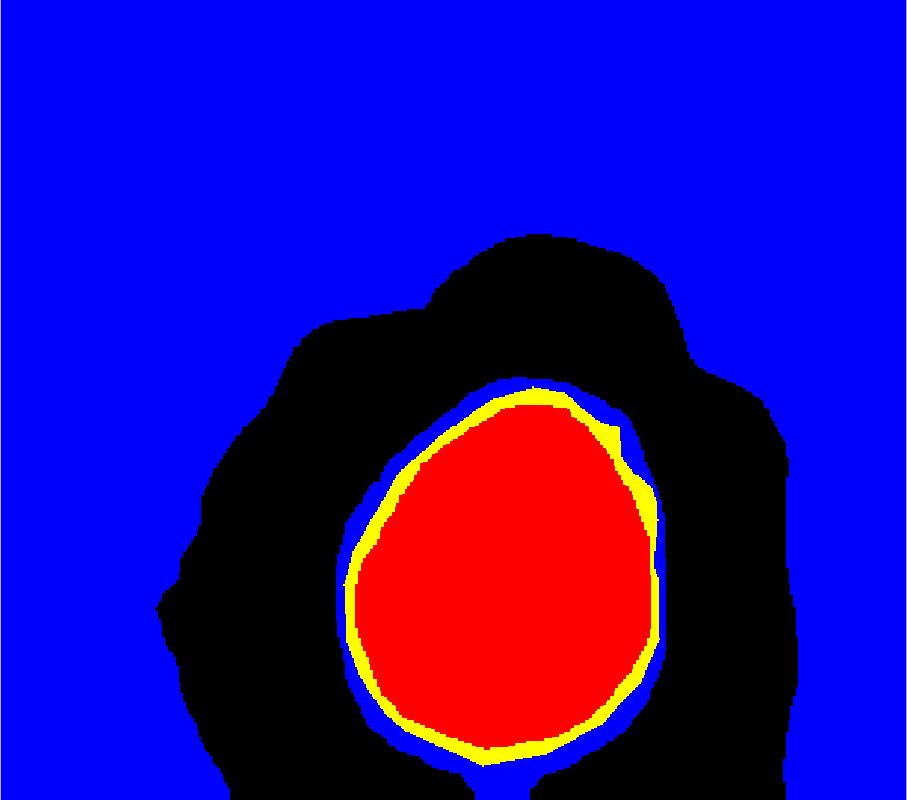
\includegraphics[width=\textwidth]{../figures/val_crs_90_orig/15.png}
		\label{fig:1}
	\end{subfigure}
	\begin{subfigure}{0.19\textwidth}
		\centering
		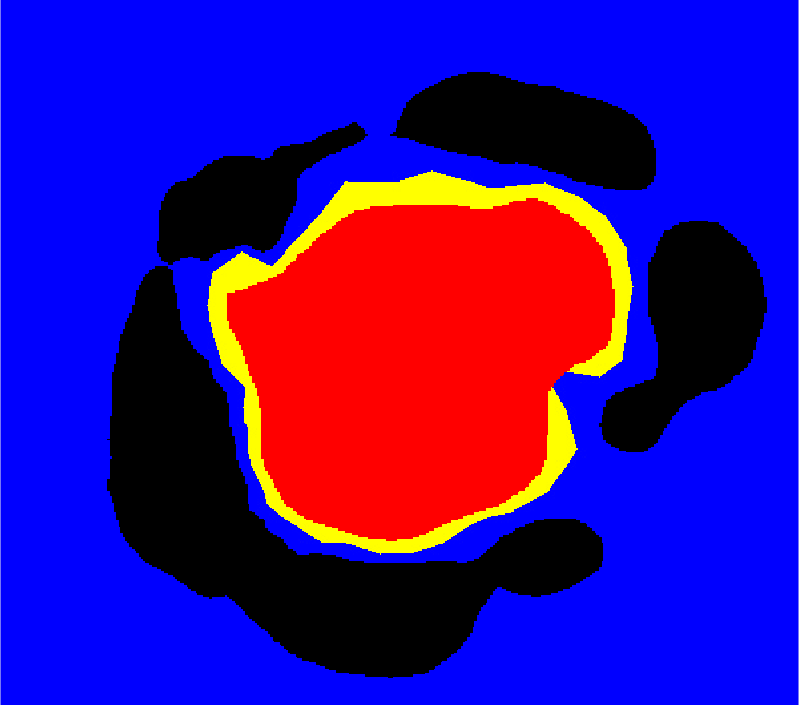
\includegraphics[width=\textwidth]{../figures/val_crs_90_orig/114.png}
		\label{fig:1}
	\end{subfigure}
	\begin{subfigure}{0.19\textwidth}
		\centering
		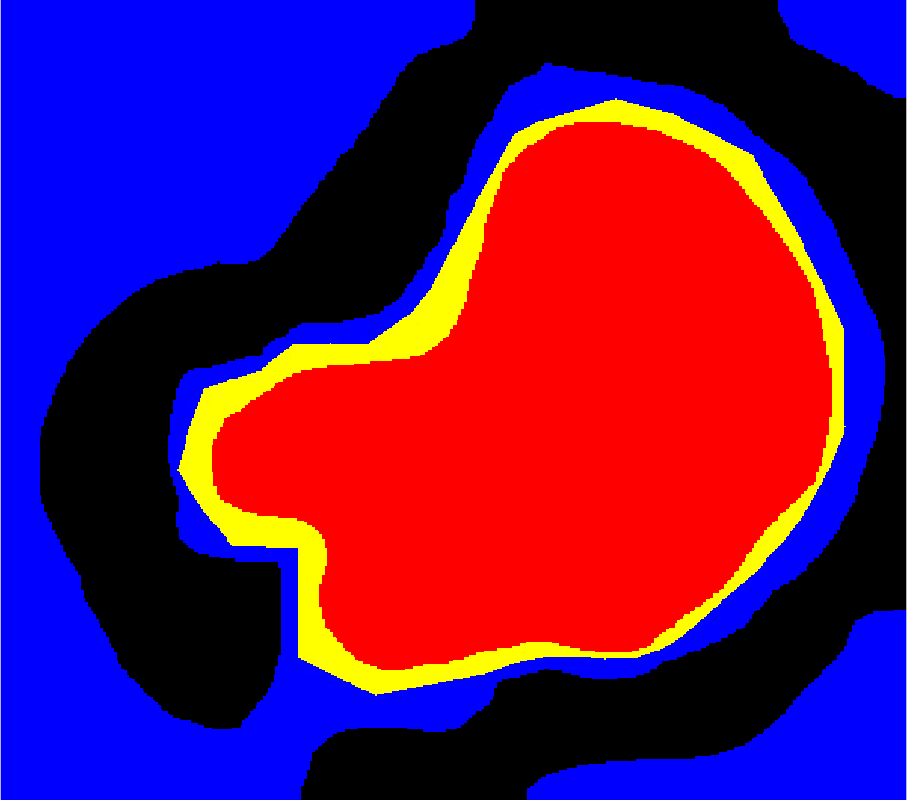
\includegraphics[width=\textwidth]{../figures/val_crs_90_orig/61.png}
		\label{fig:1}
	\end{subfigure}
	\begin{subfigure}{0.19\textwidth}
		\centering
		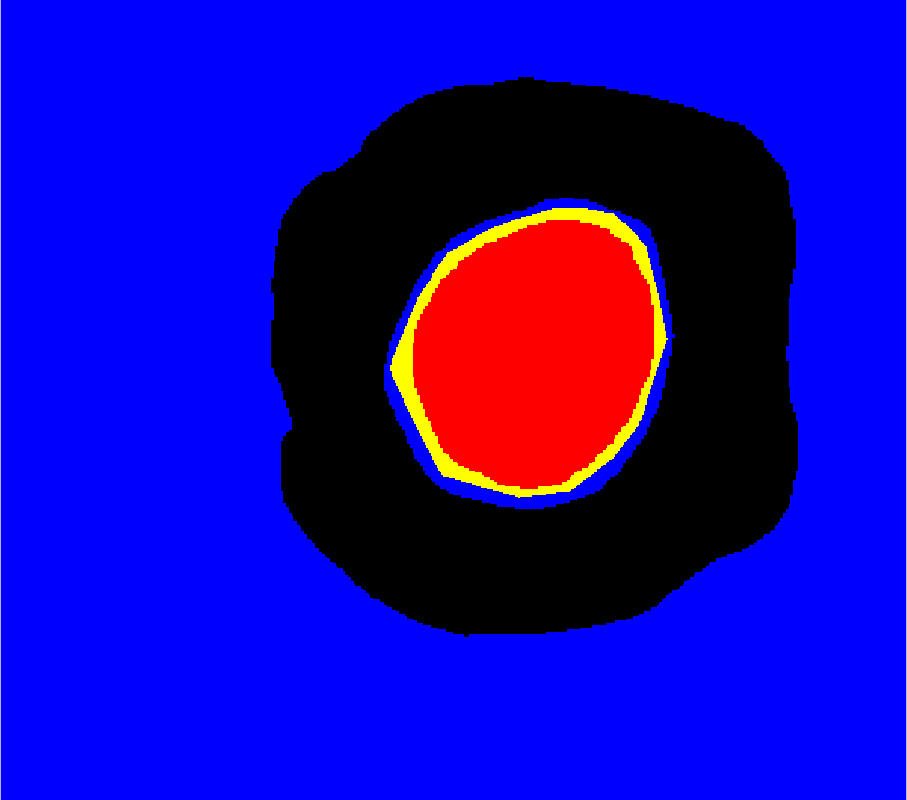
\includegraphics[width=\textwidth]{../figures/val_crs_90_orig/76.png}
		\label{fig:1}
	\end{subfigure}
	\begin{subfigure}{0.19\textwidth}
		\centering
		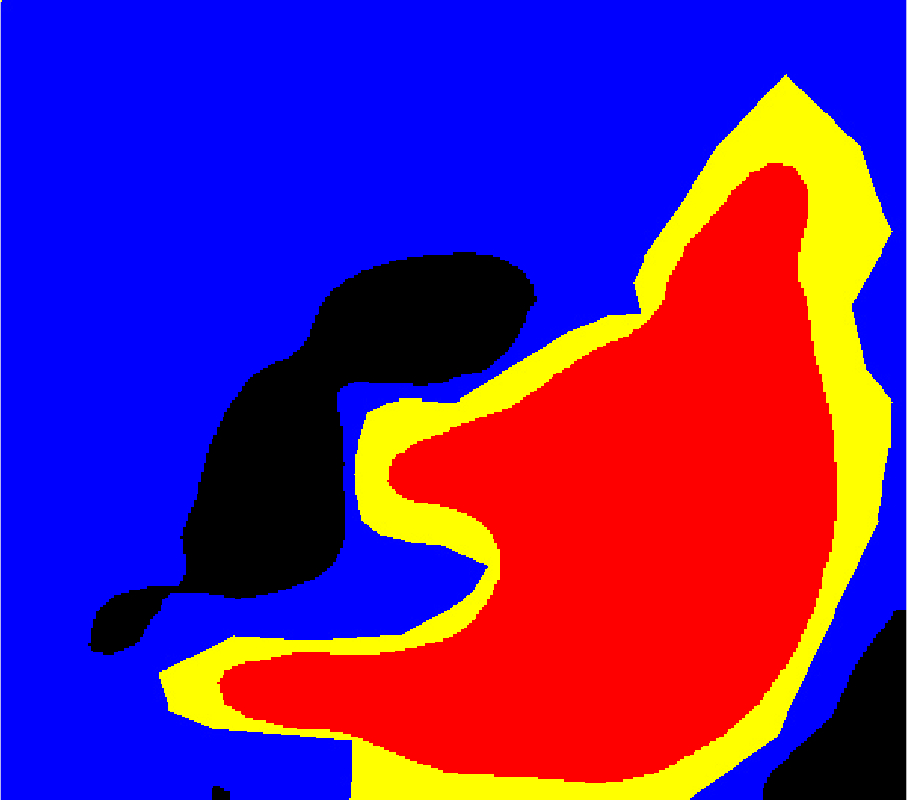
\includegraphics[width=\textwidth]{../figures/val_crs_90_orig/87.png}
		\label{fig:1}
	\end{subfigure}
		\vspace{-0.4cm}
	\\
	\begin{subfigure}{0.19\textwidth}
		\centering
		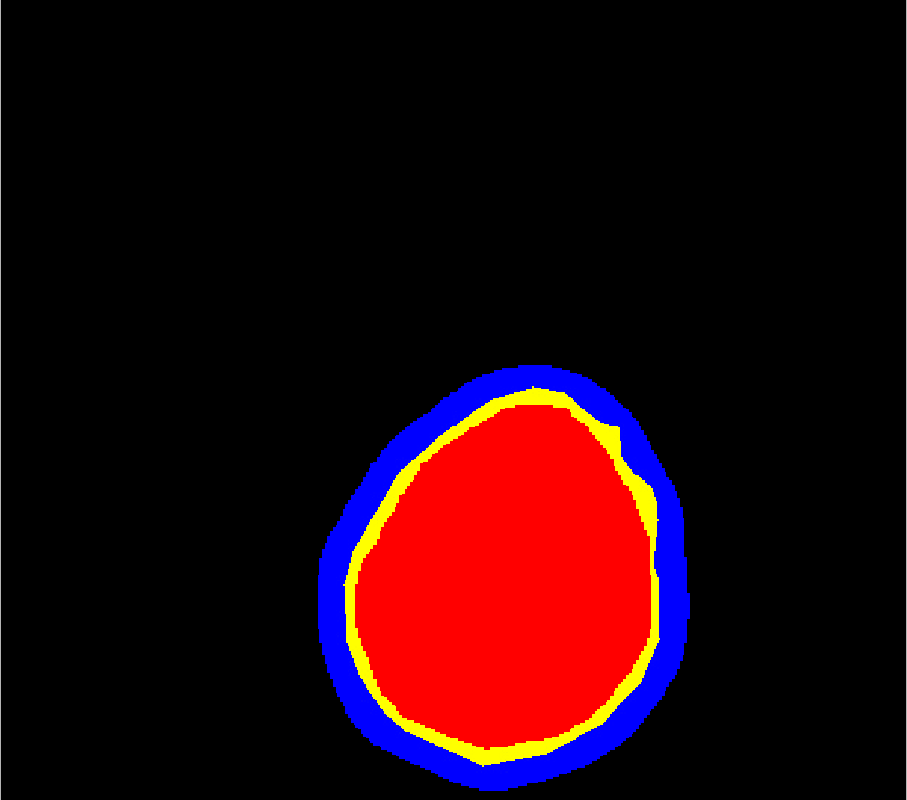
\includegraphics[width=\textwidth]{../figures/val_crs_90_distmix/15.png}
		\label{fig:1}
	\end{subfigure}
	\begin{subfigure}{0.19\textwidth}
		\centering
		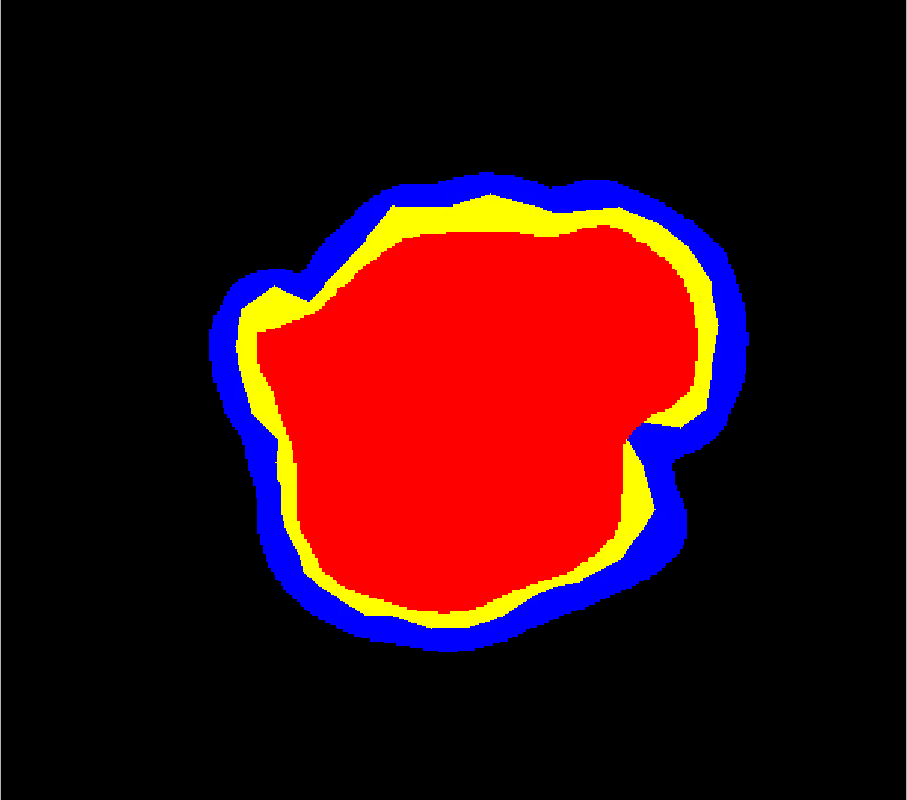
\includegraphics[width=\textwidth]{../figures/val_crs_90_distmix/114.png}
		\label{fig:1}
	\end{subfigure}
	\begin{subfigure}{0.19\textwidth}
		\centering
		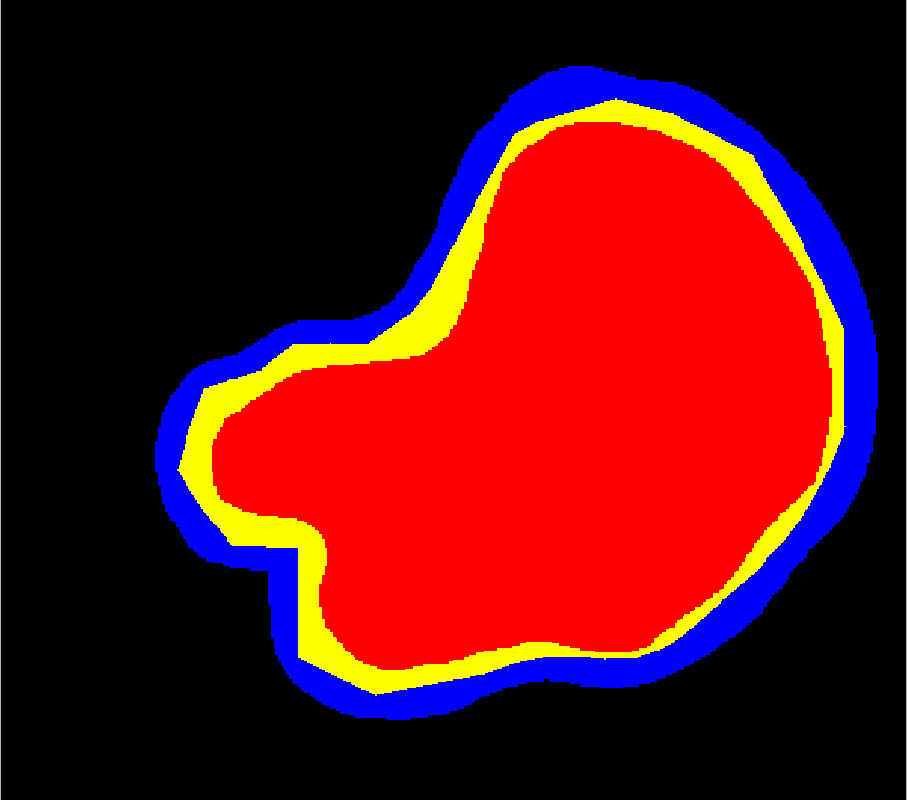
\includegraphics[width=\textwidth]{../figures/val_crs_90_distmix/61.png}
		\label{fig:1}
	\end{subfigure}
	\begin{subfigure}{0.19\textwidth}
		\centering
		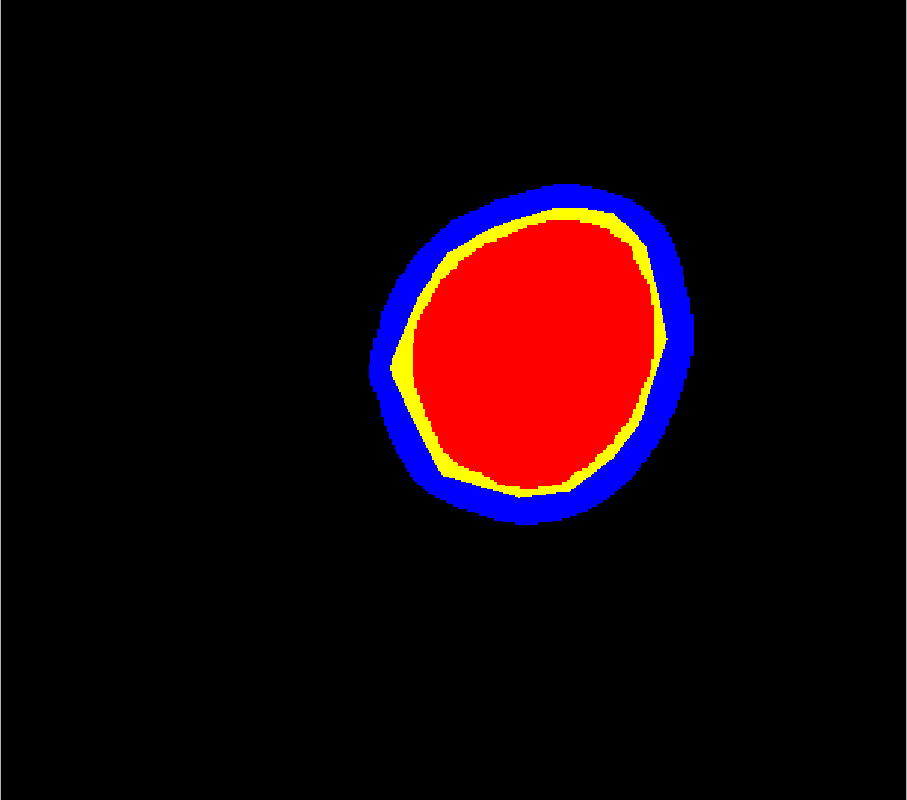
\includegraphics[width=\textwidth]{../figures/val_crs_90_distmix/76.png}
		\label{fig:1}
	\end{subfigure}
	\begin{subfigure}{0.19\textwidth}
		\centering
		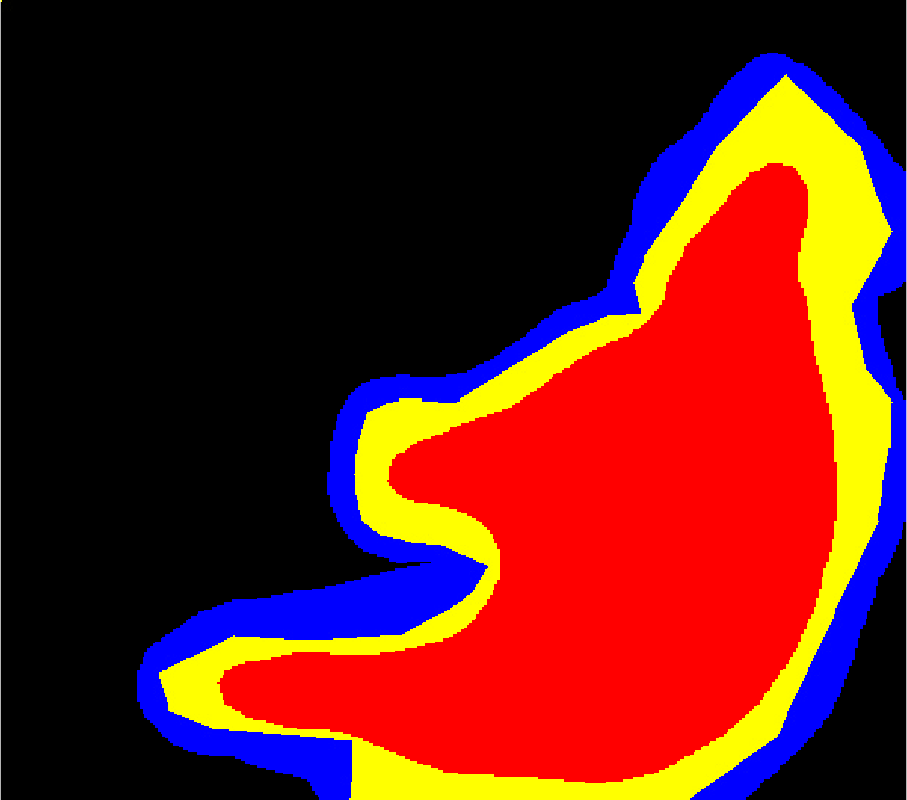
\includegraphics[width=\textwidth]{../figures/val_crs_90_distmix/87.png}
		\label{fig:1}
	\end{subfigure}
	\vspace{-0.4cm}
	\\
	\begin{subfigure}{0.19\textwidth}
		\centering
		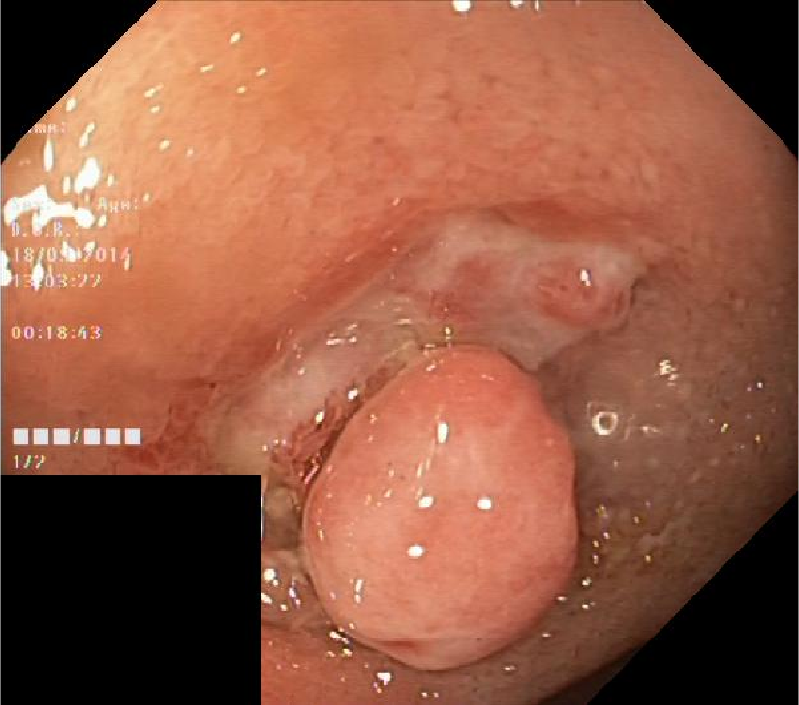
\includegraphics[width=\textwidth]{../figures/val_images/15.png}
		\label{fig:1}
	\end{subfigure}
	\begin{subfigure}{0.19\textwidth}
		\centering
		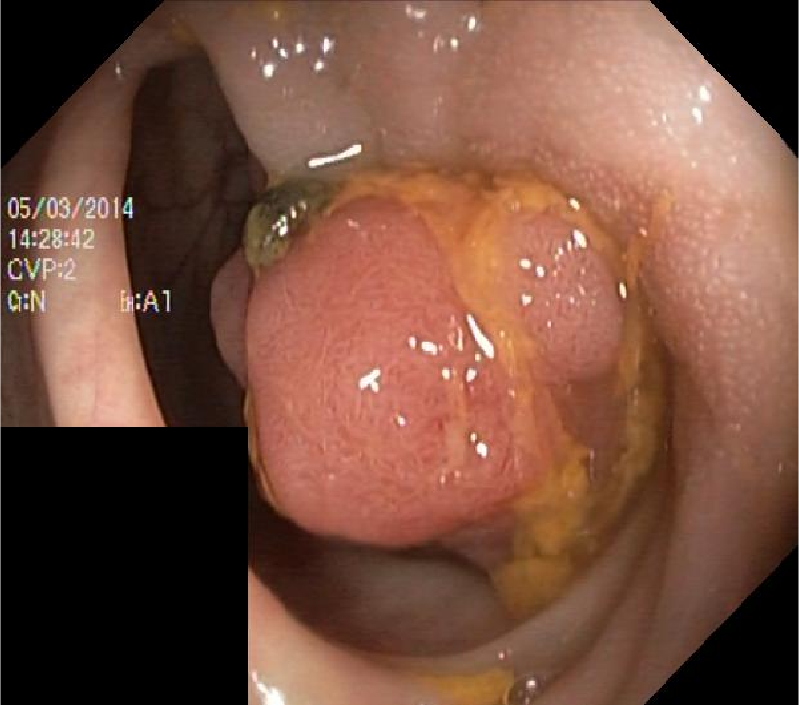
\includegraphics[width=\textwidth]{../figures/val_images/114.png}
		\label{fig:1}
	\end{subfigure}
	\begin{subfigure}{0.19\textwidth}
		\centering
		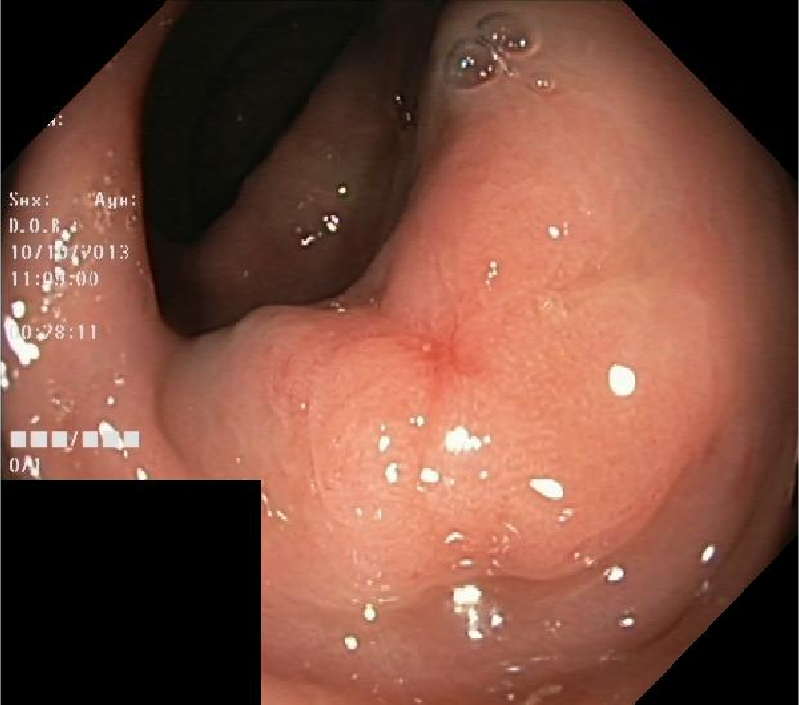
\includegraphics[width=\textwidth]{../figures/val_images/61.png}
		\label{fig:1}
	\end{subfigure}
	\begin{subfigure}{0.19\textwidth}
		\centering
		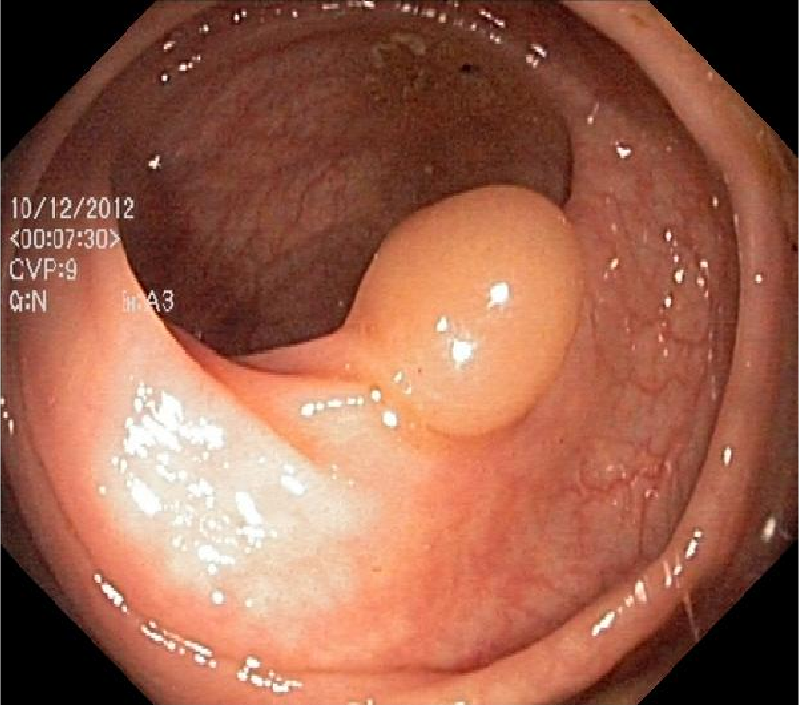
\includegraphics[width=\textwidth]{../figures/val_images/76.png}
		\label{fig:1}
	\end{subfigure}
	\begin{subfigure}{0.19\textwidth}
		\centering
		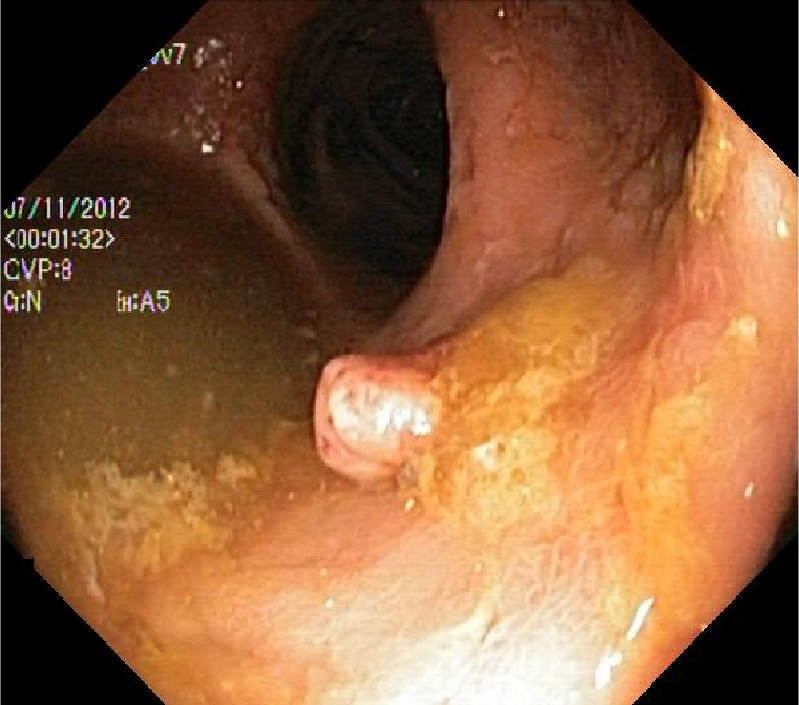
\includegraphics[width=\textwidth]{../figures/val_images/87.png}
		\label{fig:1}
	\end{subfigure}
	\label{fig:grid}
	\caption{Conformal confidence sets for the polyps data. The bottom row shows the original endoscopic images with visible polyps. The top two rows present the conformal confidence sets, with the ground truth masks shown in yellow. The inner sets and outer sets are shown in red and blue respectively. The top row illustrates the sets which arise when using the original scores. Instead the middle show the resulting sets when $f_O$ is given by the distance transformation of the predicted polpys mask. The figure shows the benefit of transforming the score function and illustrates the method's effectiveness in accurately identifying polyp regions whilst providing informative spatial uncertainty bounds.}\label{fig:polpys}
\end{figure}

\begin{figure}
	
	\caption{Left: . Right: False coverage rate of the outer and inner sets over the test set of 1000 images for $\alpha$ ranging from 0 to $0.2$.  }\label{fig:dist}
\end{figure}

The inner sets are shown in red and represent regions where we can have high confidence of the presence of polyps. The outer sets are shown in blue and represent regions in which the polpys may be.

These results show that we can provide informative confidence bounds for the location of the polpys and allow us to use the PraNet segmentation model with uncertainty guarantees. They also illustrate the limitations of the model which is essential for applications. When analyzing some images the outer uncertainty bounds can be quite large, even with the favourable alpha-weighting scheme. These images may require specialist follow-up in order to be certain about the true extent of the observed tumor. Improved uncertainty quantification would require an improved segmentation model. 

More precise results can be obtained at the expense of probabilistic guarantees, see Figure XXX. A trade off must be made between precision and confidence and this can be determined in advance based on the alpha-weighting dataset. The approach of CITE controls the empirical false negative risk yielding additional precision but at the cost of coverage as shown in Figure XXX. 

\subsection{Measuring the false coverge rate}

%\subsection{Application to Melanoma segmentation}

%\subsection{Melanoma Lesion Segmentation}

%\subsection{Melanoma Segmentation}
